\documentclass[12pt]{article}
\usepackage{currothesis}
\usepackage[left=1.5in, right=1.5in, top=1in, bottom=1in]{geometry}
\usepackage{fontspec}
%\setmainfont{Adobe Caslon Pro}
\usepackage{layout}
\usepackage[]{amsmath}
\usepackage{amssymb}
\usepackage{ragged2e}
\usepackage{graphicx}
\usepackage{cite}
\usepackage{ mathrsfs }
\usepackage{booktabs}
\usepackage{tikz}
\usepackage{caption}
\captionsetup[table]{skip=10pt}
\usetikzlibrary{matrix,chains,positioning,decorations.pathreplacing,arrows}

\DeclareMathOperator*{\argmin}{arg\,min}

\usepackage{titlesec}

\setcounter{secnumdepth}{4}

\titleformat{\paragraph}
{\normalfont\normalsize\bfseries}{\theparagraph}{1em}{}
\titlespacing*{\paragraph}
{0pt}{3.25ex plus 1ex minus .2ex}{1.5ex plus .2ex}

\def\toclevel@paragraph{4}
\setcounter{tocdepth}{4}
\pagestyle{plain}
\setlength{\marginparwidth}{1in}

\newcommand\tline[2]{$\underset{\text{#1}}{\text{\underline{\hspace{#2}}}}$}

\begin{document}

% Title page
\thispagestyle{empty}
\begin{center}
\Large

THE COOPER UNION\\
ALBERT NERKEN SCHOOL OF ENGINEERING

\vspace{1in}

{
\LARGE
A Deep Partitioned Autoencoder \\for De-Noising Live Audio

}

\vspace{1in}

by

Ethan Lusterman

\vspace*{\fill}

A thesis submitted in partial fulfillment\\
of the requirements for the degree of\\
Master of Engineering

\vspace{1in}

September 2016

\vspace{1in}

Professor Sam Keene, Advisor

\end{center}

% Signature Page
\newpage
\thispagestyle{empty}
\begin{center}
\Large
THE COOPER UNION FOR THE \\ADVANCEMENT OF SCIENCE AND ART

\vspace{0.5in}

ALBERT NERKEN SCHOOL OF ENGINEERING

\vspace{1in}

\justify

This thesis was prepared under the direction of the Candidate's Thesis Advisor
and has received approval. It was submitted to the Dean of the School of
Engineering and the full Faculty, and was approved as partial fulfillment of
the requirements for the degree of Master of Engineering.

\raggedright

\vspace{1in}

\hfill \tline{Dean, School of Engineering \hfill Date}{3in}

\vspace{1in}

\tline{Prof. Sam Keene, Thesis Advisor \hfill Date}{3in}


\end{center}

\newpage
\pagenumbering{roman}
\setcounter{page}{1}

\newpage

\begin{center}
{\Large Acknowledgements} \\

\vspace{1in}
Ack example
\end{center}

\newpage

\begin{center}
{\Large Abstract} \\

\vspace{1in}
% Traditional audio denoising systems are often linear time-invariant (LTI) and often require access to clean data to properly train to remove noise. Since clean audio is often unavailable, we build on a partitioned denoising autoencoder for denoising audio signals when clean examples are unavailable for training. In addition, the nonlinearity of a neural network architecture provides additional gains over standard linear models. We compare existing semi-supervised denoising systems as well as canonical supervised denoising autoencoders. We show that for moderate levels of noise, our autoencoder can outperform existing schemes.

In this thesis, we introduce a modified partitioned autoencoder for de-noising audio without access to clean data for training. Traditional linear time-invariant (LTI) systems such as the Wiener filter rely on power spectral density (PSD) estimates of desired signals and noise signals, which require some knowledge of the ground truth signals. One nonlinear approach in this area includes the use of de-noising autoencoders, which are one form of artificial neural networks (ANN). The nonlinearity of neural networks allow for more complex models to be made than LTI models. However, since de-noising autoencoders also require access to clean data and knowledge of the noise corruption process, we build on existing literature for a semi-supervised partitioned autoencoder that can perform de-noising without the clean signals during training. We compare existing semi-supervised de-noising systems as well as canonical supervised de-noising autoencoders. We show that for moderate levels of noise, our autoencoder outperforms existing schemes.

\end{center}


\newpage

\tableofcontents

\newpage

\listoffigures

\newpage

Table of Nomenclature

\clearpage
\setcounter{page}{1}
\pagenumbering{arabic}

\fontsize{12pt}{24pt}\selectfont
\section{Introduction}
Advances in smartphone technology have led to smaller devices with more powerful audio hardware, allowing for common consumers to make higher quality recordings. However, recorded speech and music are subject to noisy conditions, often hampering intelligibility and listenability. The goal of de-noising audio recordings is to improve intelligibility and perceived quality. A variety of applications of audio de-noising exist, including listening to a recording of a band or an artist's live performance in a noisy crowd, or listening to a recorded conversation or speech under noisy conditions.

A common technique for de-noising involves the use of autoencoder neural networks. \cite{liu2014experiments} Advances in parallel graphics processing units (GPU) and in machine learning algorithms have allowed for training deeper networks faster, utilizing more hidden layers with more neurons.

Prior work in de-noising audio has involved the use of noise-free training data. Since common consumers do not often have access to clean audio, we seek to de-noise without the use of clean audio. Other work has touched on such a semi-supervised scenario but was used more as a preprocessing step to a classification algorithm than as time-domain de-noising. \cite{stow}

In this thesis, we compare several neural network architectures and problem scenarios, ranging from data input types, level of noise, depth of network, training objectives, and more. In Chapter 2, we present background information on machine learning, neural networks, and signal processing as well as prior work in audio de-noising. In Chapter 3, we detail the problem formally as well as introduce our signal model and sourced data. In Chapter 4, we detail all considered network architectures. In Chapter 5, we compare results from different data inputs, levels of noise, network architectures, and training objectives and discuss methods of evaluation. Finally, we make conclusions and recommendations for future work in Chapter 6.

\newpage

\section{Background}
\subsection{Machine Learning}
% explain ML basics
Machine learning involves the use of computer algorithms to make decisions based on training data. Generally, this falls into categorizing input data (classification) or determining a mathetmatical function to determine a continuous output given an input (regression). Popular classification examples include recognizing handwritten digits as well as determining whether an image contains a cat or a dog. An example of a regression problem is determining the temperature given a set of input features (humidity, latitude, longitude, date, etc.).

Problems where training data contain input data vectors as well as the correct output vectors (targets) are known as supervised learning problems. Training a model to denoise audio where noise was introduced to the clean audio would be a supervised learning problem. On the other hand, training a model to denoise audio where the underlying clean signal is not known is an unsupervised learning problem. Different loss (objective) functions and neural network architectures can be exploited to accomplish denoising without the clean data.

For the purposes of this thesis, we use machine learning to determine an underlying nonlinear function that removes noise from time slices of audio (i.e. regression). These slices can then be pieced back together through overlap-add resynthesis. To clarify, this is a general linear model that maps an input noisy audio vector $y[n]=x[n]+N[n]$ to $\tilde{x}[n]$, a target denoised audio vector, where $x[n]$ is the underlying clean signal and $N[n]$ is the additive background noise.

\subsubsection{Regression}
A classical regression technique is linear regression, where one or more independent variables $x_{i}$ are used to determine a scalar dependent variable $y$. The case of a single independent variable $x$ is known as simple linear regression. More formally, for $k$ independent variables, we would like to determine a weight vector $\vec{w}$ and bias vector $\vec{b}$:

\begin{align}
y_i &= w_{1}x_{i1} + \cdots + w_{k}x_{ik} + b_{i}, \qquad i=1\ldots ,n \\
\vec{y} &= \vec{x^T}\vec{w} + \vec{b}
\end{align}

where the rows of $x^{T}$ are the example input observations and $\vec{y}$ and $\vec{b}$ are column vectors.

By extension, the case of linearly estimating a vector output giving a vector input is known as a generalized linear model. A canonical example would be estimating a sine wave $x[n]$ over some number of $N$ samples given noisy samples $y[n]=x[n]+N[n]$.


% \subsubsection{Overfitting and Curse of Dimensionality}


% \subsubsection{Loss functions and Regularization}


% \subsubsection{Gradient Stuff?}


\subsection{Neural Networks}
% Basic explanation of NN
In this thesis, we deal only with feed-forward neural networks, which are essentially directed acyclic graphs (DAG) for computation. In other words, information only moves through the network in one direction. An example neural network is shown in Figure \ref{fig:nn}.

\begin{figure}[!ht]
\centering
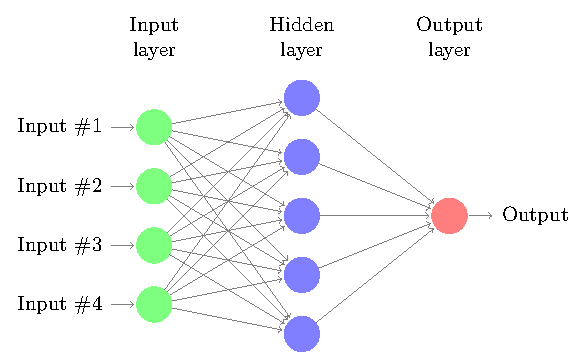
\includegraphics[width=.8\textwidth]{neural-network-texexample-net}
\caption[Example neural network]{An example neural network. There are 4 input variables, 1 hidden layer with 5 neurons, and 1 output variable. Source: http://www.texample.net/tikz/examples/neural-network/}
\label{fig:nn}
\end{figure}

The connections in a neural network can be represented by linear combinations of the input variables with learned weights $\vec{w}$. \cite{bishop} Unlike standard linear models however, neural networks apply a nonlinear activation $f(\cdot)$ at the output of each neuron. The circle nodes in a neural network diagram can be thought of as the sum of the linear combinations of the connection edges and the application of the bias and activation function. Therefore, a hidden neuron $z_{j}$ in a network with $N$ input variable nodes, $M$ hidden nodes, and $K$ output nodes takes on the value

\begin{equation}
z_j = f(a_j)
\end{equation}

where the activiation $a_j$ is given by

\begin{equation}
a_j = \sum_{i=1}^{N} w_{ji}^{(1)}x_i + w_{j0}^{(1)}
\end{equation}

The connection values $w_{ji}$ are referred to as weights, and the scalars $w_{j0}$ are referred to as biases. Note that the superscripted numbers refer to the Then, the output $y_{k}$ is given by

\begin{equation}
y_k = g(a_k)
\end{equation}

where the output activation $a{k}$ is given by

\begin{equation}
a_k = \sum_{j=1}^{M} w_{kj}^{(2)} z_j + w_{k0}^{(2)}
\end{equation}

We are free to choose activation functions, which we will discuss later. However, note that at the output, the function $g(\cdot)$ is often an identity for regression problems and a sigmoid $\sigma(\cdot)$ for classification problems.

Often, the weights and biases are grouped into a weight vector $\vec{w}$. In other words, similar to the linear models described earlier, a neural network is a nonlinear function of input variables $\{x_i\}$ to output variables $\{y_k\}$ where the parameters of the function are learned via training techniques.

\subsubsection{Dense Layer}

Described in the previous section, we refer to a dense layer as a fully connected neural network, in which no interconnections between neurons are missing at each layer. Dense layers can be prone to overfitting. However, as we mention later, overfitting is not an immediate concern for the purposes of this thesis.

\subsubsection{De-noising Autoencoder}

An autoencoder is normally an abstraction of neural networks in which an encode function $\vec{Z}=f(\vec{X})$ and a decode function $\hat{\vec{X}}=g(\vec{Z})$ are learned to learn a lower-dimensional representation of some input $\vec{X}$. \cite{stow} A de-noising autoencoder is a supervised process whereby the clean input is first corrupted by some stochastic process $\vec{Y}=u(\vec{X})$. In other words, the neural network input would be a noisy input $Y$, and the network would try to learn weights such that the network output $\vec{\hat{X}}$ approximates the clean input $\vec{X}$. Another way to frame it is that your network is learning the inverse function of the noise process $u(\vec{x})$.

% \subsubsection{Convolutional Layer}



\subsubsection{Network Training}

In order to train a neural network, we must update the weights such that we minimize a loss function, often some kind of sum-of-square error function. \cite{bishop} Often, a stochastic gradient descent (SGD) approach is taken to determine the weights that minimize the loss function.



% \subsubsection{Regularization}



\subsubsection{Choice of Activation Function}

The most common activation functions used are the logistic sigmoid function and the hyperbolic tangent. \cite{liu2014experiments} The logistic sigmoid function is given by

\begin{equation}
g(x) = \dfrac{1}{1+\exp{(-x)}}
\end{equation}

Note that the sigmoid function has an output on the range $(0,1)$. The hyperbolic tangent function (tanh) is given by

\begin{align}
g(x) &= \dfrac{\sinh{x}}{\cosh{x}}\\
&= \dfrac{\exp{(x)}-\exp{(-x)}}{\exp{(x)}+\exp{(-x)}}\\
&= \dfrac{1-\exp{(-2x)}}{1+\exp{(-2x)}}
\end{align}

Note that the hyperbolic tangent function has an output on the range $(-1,1)$.

Generally, our choice of nonlinearity should be chosen such that the expected range of desired output matches the nonlinearity's. In the case of audio de-noising, different activations can be chosen depending on the input format. For example, time-domain audio frames are often processed with a digital floating point representation on the range of $[-1,1]$. In such a case, the hyperbolic tangent might be appropriate. On the other hand, if we were working with magnitude spectra of an audio signal, we would use a linearity with an output range of $[0,\infty]$.

Recently, a more popular activation function which has in use is the rectified linear unit (ReLU). \cite{glorot2011deep} The ReLU is defined by the following:

\begin{equation}
g(x) =
    \begin{cases}
        \hfill 0 & \text{if $x < 0$}\\
        \hfill x & \text{if $x \ge 0$}
    \end{cases}
\end{equation}

In other words, $g(x)=\max{(0,x)}$. This function satisfies the range of output we expect for magnitude spectra. In terms of gradient calculations, the zero derivative for negative input values of $x$ can cause nodes to not be activated, potentially leading to gaps in information at the output and slower training time. To combat this, variations of the ReLU are used which have small, non-zero gradients for negative input values. For example, leaky ReLU's are defined by

\begin{equation}
g(x) =
    \begin{cases}
        \hfill 0.01x & \text{if $x < 0$}\\
        \hfill x & \text{if $x \ge 0$}
    \end{cases}
\end{equation}

Advantages of ReLU's include better gradient propagation as well as fast computation and sparse representation. Some disadvantages include non-differentiability at $x=0$. Also, depending on use case, sparse representation might not be desired.

\subsubsection{Minibatch Training}

Historically, neural networks were trained one example at a time (online) or in a batch (all examples at once). \cite{wilson2003general} For the online approach, the network weights are updated after gradients are calculated and backpropagated for each training example. On the other hand, the batch approach accumulates average gradients for all examples and then updates the network weights. The batch approach might approximate the true gradients better than the online approach, but the online approach tends to have faster training time and convergence. \cite{wilson2003general} This is because with an online approach, the network is less likely to get stuck in a local minimum.

Minibatch training has become more popular recently. Serving as a midway point between the two approaches, minibatch training exposes the network to a small number of examples and then accumulates gradients and updates the network weights. The trend toward minibatch training comes at a time where parallel computing resources are easily accessible.


\subsubsection{Batch Normalization}

Batch normalization is a technique that helps to speed up training time and convergence. Batch normalization accumulates learned statistics of the network to help achieve loss convergence more quickly. More formally, an input minibatch $x$ is normalized by the following:

\begin{equation}
y = \dfrac{x-\mu}{\sqrt{\sigma^{2}+\epsilon}}\gamma + \beta
\end{equation}

\cite{ioffe2015batch}. During training, the minibatches are normalized to zero-mean, unit-variance and transformed by parameters $\gamma$ and $\beta$. At inference time, the learned parameters are instead used, which are made up of the average statistics from training.

Batch normalization prevents activations from saturating from widely varying input minibatches. This allows us to use faster learning rates and be less careful about how to initialize our parameters. \cite{ioffe2015batch}

\subsection{Signals and Systems}
Domain knowledge of discrete audio signals and systems better informs our decisions for an audio denoising system, so some background information on signals and systems as it pertains to this thesis is detailed below.

\subsubsection{Signals}
We deal exclusively with discrete-time audio signals in this thesis. A discrete-time audio signal $x[n]$ is represented as a sequence of numbers (samples), where each integer-valued slot $n$ in the sequence corresponds to a unit of time based on the sampling frequency $f_s$. This comes from sampling the continuous-time audio signal $x_c(t)$:

\begin{equation}
x[n] = x_c(nT)
\end{equation}

where $T=1/f_s$.
For example, a 1-second speech signal sampled at 8kHz has 8000 samples. Furthermore, digital signals also have discrete valued sample amplitudes. For the purposes of this thesis, the bit depths of computers we use for analysis are high enough to allow for perfect reconstruction between continuous-time signals and digital signals.

We also assume signals collected have been properly sampled according to the Nyquist-Shannon sampling theorem, which states that a discrete-time signal must be sampled at at least twice the highest frequency present in the signal to prevent aliasing of different frequencies. For example, speech signals genearlly have information up to 8kHz, so many speech signals are sampled at 16kHz. Music is more complex in that signals often span up to about 20kHz, so CD quality recordings are often sampled at 44.1kHz or higher. For this thesis, we use recordings sampled at 44.1kHz or lower.


\subsubsection{Convolution} % TODO: figure with basic flip/slide convolution
The discrete-time convolution operation takes two sequences $x[n]$ and $h[n]$ and outputs a third sequence $y[n] = x[n] * h[n]$:

\begin{equation}
y[n] = \sum_{k=-\infty}^{\infty} x[k]h[n-k]
\end{equation}

Convolution is commutative, so $x[n] * h[n] = h[n] * x[n]$ holds true.

A linear, time-invariant (LTI) system is characterized by its impulse response $h[n]$, which allows us to determine samples $y[n]$ when $x[n]$ is subject to $h[n]$. For the purposes of this thesis, our underlying clean signal $x[n]$ might be subject to the conditions of an acoustic environment $h[n]$ and crowd noise $N[n]$:

\begin{equation}
y[n] = h[n]*x[n]+N[n]
\end{equation}

In this scenario, our system would attempt to recover $h[n]*x[n]$ and possibly even $x[n]$ if the acoustic environment were deemed ``noisy enough'' due to echo and reverberation.

One of our proposed systems also incorporates convolutional neural networks (CNN) which use convolutions between frames of samples instead of simple linear combinations (discussed later).

\subsubsection{Frequency Transforms} % TODO: figure with time and frequency graph
In some of our proposed systems, we use a frequency transformed version of the input signal as a preprocessing step to the system input. While no new information is gained from transforming the input, networks often respond better to determining the value of the magnitude of varying frequencies at a time slice instead of the individual time samples.

The frequency transform we use in this thesis is the discrete-time Fourier transform (DTFT). A sequence of $N$ discrete-time samples is transformed into another sequence of $N$ samples where each index then corresponds to a frequency bin. The DTFT $X[k]$ of a signal $x[n]$ is given by the following:

\begin{equation}
X[k] = \sum_{n=0}^{N-1} x[n] W_N^{kn}
\end{equation}

where the twiddle factor $W_N$ is given by $W_N=e^{-j(2\pi/N)}$. Then the reconstruction of $x[n]$ from $X[k]$ is given by:

\begin{equation}
x[n]=\dfrac{1}{N} \sum_{k=0}^{N-1} X[k] W_N^{-kn}
\end{equation}

In this thesis, we also exploit the main duality between the time and frequency domain using the convolution theorem, which states that convolution in time is equivalent to multiplication in frequency and vise versa:

\begin{equation}
\mathscr{F} \{h[n] * x[n]\} = H[k] X[k]
\end{equation}
\begin{equation}
\mathscr{F}^{-1} \{H[k] * X[k]\} = h[n] x[n]
\end{equation}

This allows us to effectively treat our network as a non-linear filter that can denoise small time/frequency slices of our noisy signal, which can then be pieced back together using overlap-add resynthesis. We detail this in the next section.

\subsubsection{Windowing and Perfect Reconstruction}



\subsubsection{Noise and Signal-to-Noise Ratio}

\newpage

\section{System Description}
\newpage


\section{Results}
We present results here for mainly shallow network architectures. At the output layer of each network, an identity nonlinearity is used. At any other layer, the modified ReLU (mReLU) is used. Unless otherwise noted, batch normalization is applied at the input layer. Each network is compared first to itself at varying noise levels (-6 dB, -3 dB, 0 dB, 3 dB, 6 dB SNR) in terms of convergence as well as the mean squared error (MSE) for inferences.

Training minibatches consist of 128 examples, each with 1024-sample FFT frames of $\norm{Y[k]}$ at a sampling rate 16 kHz. Time windows are windowed using the Hanning window, and we use 50\% overlap for perfect reconstruction at inference time. The examples used are a sum of sine waves at four fixed frequencies with uniform random amplitude and phase. The frequencies are chosen to form an A4 major chord (1-3-5-8) at slightly de-tuned frequencies so as not to allow the network to learn any pattern from the immediate harmonic structure.

\begin{align}
f &= [441, 549, 660, 881]\qquad \text{Hz}\\
x[n] &= \sum_{i=0}^{3} A_i \sin{2 \pi f_i / f_s n + \phi_i}, \qquad n=0,\ldots ,1023\\
A_i &\sim U(0.25, 0.75)\\
\phi &\sim U(0, 2\pi)
\end{align}

Applied noise is additive-white Gaussian noise (AWGN), with the variance $\sigma^2$ selected to achieve the desired average SNR for each minibatch as in Equation \ref{eq:siggy}.

\begin{align}
N[n] &\sim N(0, \sigma^2), \qquad n=0,	\ldots ,1023\\
y[n] &= x[n] + N[n]
\end{align}

In semi-supervised cases where we use the soft label $y$ for noise-only versus signal-plus-noise examples, we use 25\% noise-only examples per minibatch. For inference calculations, we construct a minibatch with consecutive overlapping, windowed frames.

Simulations are written in Python 2.7 using Lasasgne \cite{sander_dieleman_2015_27878}, a ``lightweight library to build and train neural networks in Theano.'' Theano is a ``Python library that allows you to define, optimize, and evaluate mathematical expressions involving multidimensional arrays efficiently.'' \cite{2016arXiv160502688short} Theano boasts parallel GPU support, Numpy support (a mathematical Python library), numerical stability, and symbolic differentiation, among other features. These libraries and frameworks allow for ease of developing deep, novel architectures and save time in doing things like calculating gradients, weight updates and back-propagation. Sample simulation code is shown in the Appendix.

Weight updates are calculated using Adam updates \cite{DBLP:journals/corr/KingmaB14}. 2000 iterations (minibatches) are used for each simulation. Unless otherwise noted, each hidden layer uses 2000 hidden nodes.

Loss-based plots show the loss function convergence during training iterations, where the loss function is as defined in the previous section for each network architecture. Mean squared error plots show the MSE every 50 training examples for an inference example that does not change.

\subsection{Supervised Autoencoder}

The following results show a single-layer autoencoder with and without batch normalization at the input layer. We present these to compare the effects of batch normalization as well as to show the differences between supervised and semi-supervised de-noising approaches.

\subsubsection{Batch Normalized Input}

In Figure \ref{fig:paris-bn-loss}, we can see that the loss function appears to converge at or before 2000 iterations. As expected, as SNR increases, the loss objective converges to a lower value. Since this network is trained using only the squared error loss, this should be expected. Note that as the SNR increases, the difference in the converged value gets smaller. Also interesting is the fact that lower SNR plots converge more quickly but to higher values. This suggests that the network does not respond well to too much noise.

\begin{figure}[!ht]
\centering
\includegraphics[width=.8\textwidth]{../thesis/thesis/comparisons/plotfinal/pdf/paris-loss}
\caption{Loss at various SNRs for Supervised Single-Layer Autoencoder with Batch Normalization at the Input}\label{fig:paris-bn-loss}
\end{figure}

In Figure \ref{fig:paris-bn-mse}, we can see that the MSE generally goes down as SNR goes up. This should be expected, though perhaps there may be an error in the simulation since the lines blur a bit between -3 dB and 6 dB.

We also note from personal listening tests that the reconstructed signals have some distortion introduced from the network.

\begin{figure}[!ht]
\centering
\includegraphics[width=.8\textwidth]{../thesis/thesis/comparisons/plotfinal/pdf/paris-mse}
\caption{MSE at various SNRs for Supervised Single-Layer Autoencoder with Batch Normalization at the Input}\label{fig:paris-bn-mse}
\end{figure}

\subsubsection{Non-Batch Normalized Input}

As expected, in Figure \ref{fig:paris-loss}, the loss metric converges about the same as for the batch normalized case. As expected, the convergence time in terms of number of iterations is slightly higher. One interesting section is how the 6 dB curve converges. It appears to have a strong section of downward concavity. It is possible that this occurred randomly, as the random number generator in Numpy was set to a random seed. It is also possible that because of an absence of batch normalization, some neurons saturated and did not change substantially for some time.

\begin{figure}[!ht]
\centering
\includegraphics[width=.8\textwidth]{../thesis/thesis/comparisons/plotfinal/pdf/paris-nobatchnorm-loss}
\caption{Loss at various SNRs for Supervised Single-Layer Autoencoder without Batch Normalization at the Input}\label{fig:paris-loss}
\end{figure}

The MSE in Figure \ref{fig:paris-mse} converges to a lower value than that of Figure \ref{fig:paris-bn-mse}. This suggests that there may be an error in the simulation, likely in using the stored statistics for batch normalization as opposed to using an on-the-fly calculation of the minibatch statistics at inference time. Batch normalization usually allows for faster convergence of the loss function. This may suggest that the mean squared error of the magnitude FFT coefficients are not as directly correlated to the time-domain signal mean squared error convergence. However, we still achieve convergence here which is expected. Past 0 dB, the MSE seems to converge to a similar value, suggesting that the network has diminishing returns for higher SNR.

\begin{figure}[!ht]
\centering
\includegraphics[width=.8\textwidth]{../thesis/thesis/comparisons/plotfinal/pdf/paris-nobatchnorm-mse}
\caption{MSE at various SNRs for Supervised Single-Layer Autoencoder without Batch Normalization at the Input}\label{fig:paris-mse}
\end{figure}


\subsection{Partitioned Autoencoder}

For the dense partitioned autoencoder, the loss function appears to converge although at a slower rate in Figure \ref{fig:dan-loss}. The loss function also converges to a higher magnitude value since the network is not supervised. In addition, the large regularization term in the loss function defined in Equation \ref{eq:stowloss} contributes to the higher convergence values for the simulation. 

\begin{figure}[!ht]
\centering
\includegraphics[width=.8\textwidth]{../thesis/thesis/comparisons/plotfinal/pdf/dan-dense-loss}
\caption{Loss at various SNRs for Single-Layer Partitioned Autoencoder\cite{stow}}
\label{fig:dan-loss}
\end{figure}

The MSE is surprisingly low in Figure \ref{fig:dan-mse}. Unlike in the supervised case, the MSE seems to spread out more as SNR increases. Even at 0 dB, the network seems to learn the noise to some success. A listening test indicates noticeably lower noise level with minimal introduced distortion.

\begin{figure}[!ht]
\centering
\includegraphics[width=.8\textwidth]{../thesis/thesis/comparisons/plotfinal/pdf/dan-dense-mse}
\caption{MSE at various SNRs for Single-Layer Partitioned Autoencoder\cite{stow}}
\label{fig:dan-mse}
\end{figure}

\subsection{Partitioned Curro Autoencoder}

For the Curro Autoencoder simulation, we used 2 dense layers of size 2048 each before partitioning into two 1024 networks. After the partition, we used two dense layers and an output layer for both partitions, all at size 1024.

Interesting to note for the Curro Autoencoder is the fact that it converges almost as quickly across SNR, which can be seen in Figure \ref{fig:curro-loss}. This suggests that the network might have a lesser dependence on SNR than for the other networks. For a real-time systems application, this suggests that the Curro network could outperform the Dense Partitioned Autoencoder. On the other hand, this could suggest that the network quickly gets stuck in a local minimum and fails to reach lower convergence.

\begin{figure}[!ht]
\centering
\includegraphics[width=.8\textwidth]{../thesis/thesis/comparisons/plotfinal/pdf/curro-loss}
\caption{Loss at various SNRs for Single-Layer Curro Autoencoder}\label{fig:curro-loss}
\end{figure}

In Figure \ref{fig:curro-mse}, for -6 dB, the time-domain MSE seems to go up slightly after 50-100 iterations, suggesting that either the loss function or the reconstruction could be incorrect. As expected, the network performs better for higher SNR but still seems to get diminishing returns for SNRs greater than 0 dB.

The plot shows the MSE for reconstruction using only the signal half of the network, i.e. the top half. Interestingly, a listening test indicates that summing the two partitions at the output seems to produce a lower noise volume and lower distortion than for either partition individually. This suggests that the network might not be properly partitioning. It is currently unclear as to whether or not this is the result of a bug in the code or a fundamental flaw in the network architecture. Since this network does not have additional dense layers at the summed output, it could be that the network needs to be deeper.

Another possibility is that the underlying symmetry in the FFT is causing the network to effectively initialize to two parallel networks. This could be mitigated by only using the first half of the FFT. Also, adding batch normalization to the rest of the layers might result in better convergence and performance.

\begin{figure}[!ht]
\centering
\includegraphics[width=.8\textwidth]{../thesis/thesis/comparisons/plotfinal/pdf/curro-mse}
\caption{MSE at various SNRs for Single-Layer Curro Autoencoder}\label{fig:curro-mse}
\end{figure}

\subsection{Comparison of Loss Convergence}

A comparison of loss functions is not reasonable 
Since our networks have different loss functions, it does not make sense to compare them based on the converged value. Rather, we would like to compare the networks for convergence time in terms of number of iterations, i.e. number of minibatches exposed to the network. From previous figures, we should expect that the SNR might have some difference depending on the network.

\begin{figure}[!ht]
\centering
\includegraphics[width=.8\textwidth]{../thesis/thesis/comparisons/plotfinal/pdf/comparison-loss--6}
\caption{Loss Comparison of Various Networks at -6 dB}\label{fig:comp-loss--6}
\end{figure}

\begin{figure}[!ht]
\centering
\includegraphics[width=.8\textwidth]{../thesis/thesis/comparisons/plotfinal/pdf/comparison-loss--3}
\caption{Loss Comparison of Various Networks at -3 dB}\label{fig:comp-loss--3}
\end{figure}

\begin{figure}[!ht]
\centering
\includegraphics[width=.8\textwidth]{../thesis/thesis/comparisons/plotfinal/pdf/comparison-loss-0}
\caption{Loss Comparison of Various Networks at 0 dB}\label{fig:comp-loss-0}
\end{figure}

\begin{figure}[!ht]
\centering
\includegraphics[width=.8\textwidth]{../thesis/thesis/comparisons/plotfinal/pdf/comparison-loss-3}
\caption{Loss Comparison of Various Networks at 3 dB}\label{fig:comp-loss-3}
\end{figure}

\begin{figure}[!ht]
\centering
\includegraphics[width=.8\textwidth]{../thesis/thesis/comparisons/plotfinal/pdf/comparison-loss-6}
\caption{Loss Comparison of Various Networks at 6 dB}\label{fig:comp-loss-6}
\end{figure}

In Figures \cref{fig:comp-loss--6,fig:comp-loss--3,fig:comp-loss-0,fig:comp-loss-3,fig:comp-loss-6}, the Curro Autoencoder seems to converge the quickest, followed by the two supervised networks, then the Dense Partitioned Autoencoder converging the slowest. As expected, as SNR goes up, the supervised networks converge slower while the semi-supervised networks seem to not be as effected by SNR.


\subsection{Comparison of Mean Squared Error Convergence}

In terms of MSE convergence, we can safely compare both the convergence time and the value of convergence since the reconstruction is based on the same inference example.

\begin{figure}[!ht]
\centering
\includegraphics[width=.8\textwidth]{../thesis/thesis/comparisons/plotfinal/pdf/comparison-mse--6}
\caption{MSE Comparison of Networks at -6 dB}\label{fig:comp-mse--6}
\end{figure}

\begin{figure}[!ht]
\centering
\includegraphics[width=.8\textwidth]{../thesis/thesis/comparisons/plotfinal/pdf/comparison-mse--3}
\caption{MSE Comparison of Networks at -3 dB}\label{fig:comp-mse--3}
\end{figure}

\begin{figure}[!ht]
\centering
\includegraphics[width=.8\textwidth]{../thesis/thesis/comparisons/plotfinal/pdf/comparison-mse-0}
\caption{MSE Comparison of Networks at 0 dB}\label{fig:comp-mse-0}
\end{figure}

In Figures \cref{fig:comp-mse--6,fig:comp-mse--3,fig:comp-mse-0}, we see that at low SNR the Dense Partitioned Autoencoder usually has the highest MSE. We expect the supervised autoencoders to have lower MSE, which is the case for these figures. However, the Curro Autoencoder has better performance than the supervised systems which is somewhat unexpected. We should expect that the network which has access to the ground truth during training should converge to a lower MSE. This could be a simulation error and is an important area of future research.

\begin{figure}[!ht]
\centering
\includegraphics[width=.8\textwidth]{../thesis/thesis/comparisons/plotfinal/pdf/comparison-mse-3}
\caption{MSE Comparison of Networks at 3 dB}\label{fig:comp-mse-3}
\end{figure}

\begin{figure}[!ht]
\centering
\includegraphics[width=.8\textwidth]{../thesis/thesis/comparisons/plotfinal/pdf/comparison-mse-6}
\caption{MSE Comparison of Networks at 6 dB}\label{fig:comp-mse-6}
\end{figure}

Also interesting to note is that for higher SNR, the Partitioned Dense Autoencoder outperforms both supervised methods. This can be seen in Figures \cref{fig:comp-mse-3,fig:comp-mse-6}. If the results are correct, this suggests that a semi-supervised network can outperform a supervised network. This might be the result of enforcing a structure of the latent space, whereas normally differences in initialization of parameters can cause vastly different latent representations.

Also interesting is the fact that for the highest SNR 6 dB, the Partitioned Dense Autoencoder outperforms the Curro Autoencoder. This can be seen in Figure \ref{fig:comp-mse-6}. Again, this could be the result of a simulation error or it could suggest that the Dense Partitioned Autoencoder performs well at high SNR.

\newpage


\section{Conclusions and Future Work}
\subsection{Conclusions}
Deep partitioned neural network architectures using time and frequency input data seem promising in long-term solutions for denoising speech and music signals. Future work is detailed in the next section.

\subsection{Future Work}
\subsubsection{Models}
The simulations can easily be extended to multiple hidden layers. These layers can be a combination of convolutional layers as well as fully connected layers. \cite{kayserdenoising} Other recent literature has pointed to recurrent neural networks as an advanced technique for de-noising which has had some success. \cite{graves2014towards} Batch normalization and layer normalization techniques can help speed up convergence in terms of wall time as well as number of minibatch iterations. \cite{2016arXiv160706450L}

Additionally, the partitions can potentially be constructed to have varying degrees of signal/noise energy such that a more gradual de-noising can occur with less distortion. The partitions can also potentially span more than one layer, which might produce interesting results. Results can then be presented in terms of additional learned parameters which dictate how much of each latent variable to use in reconstruction.

Other metrics could be useful as well in reporting results besides Mean Squared Error. For instance, we could measure the signal-to-distortion ratio (SDR) to identify which networks are introducing distortion and which ones are preventing it. We could also modify our MSE to report as a gain in SNR instead. If we want to preserve audio quality and measure it, we could potentially use user listening tests and audio quality metrics which are based on perceptual models of human hearing.

It's also worth exploring whether or not these models might generalize to similar situations of noisy conditions but with different signals, or vise versa.

\subsubsection{Data}
Various data sources could be considered in validating the various presented network architectures. Different signal types, e.g. various speech examples and music recordings could provide more useful insights across models and simulations. Similarly, different noise signal types, e.g. restaurant noise, train noise, and crowd noise could provide more insight into how the networks respond.


\newpage

\nocite{*}
\fontsize{12pt}{16pt}\selectfont
\bibliography{bib}{}
\bibliographystyle{IEEEtran}

\end{document}
